\documentclass[letterpaper,twocolumn,10pt]{article}
\usepackage{usenix2019_v3}

% to be able to draw some self-contained figs
\usepackage{tikz}
\usepackage{amsmath}
\usepackage{float}

% inlined bib file
\usepackage{filecontents}

%-------------------------------------------------------------------------------
\begin{filecontents}{references.bib}
%-----------------------------------------------------------------------

\end{filecontents}

%-------------------------------------------------------------------------------
\begin{document}
%-------------------------------------------------------------------------------

%don't want date printed
\date{}

% make title bold and 14 pt font (Latex default is non-bold, 16 pt)
\title{\Large \bf Extending ZenFS: Striped SSTable Placement and Proactive Reclaim for ZNS-Aware RocksDB}

%for single author (just remove % characters)
\author{
{\rm Kitty Wang}\\
School of Engineering and Applied Sciences\\
  Harvard University\\
  Cambridge, MA 02134 \\
  \texttt{kittywang@college.harvard.edu} \\
} % end author

\maketitle


%-------------------------------------------------------------------------------
\section{Introduction}
Log-structured merge-tree (LSM-tree) key-value stores have become widely deployed in data-intensive systems as they transform random updates into sequential persistent writes. RocksDB is a prominent example as a LSM-tree key-value store whose storage behavior is dominated by immutable sorted string table (SSTable) files. Writes are appended to a write-ahead log, inserted into an in-memory memtable, and later flushed to storage as immutable sorted string table (SSTable) files. Background compaction subsequently reads existing SSTables, merges overlapping key ranges, removes obsolete entries, and writes new SSTables \cite{dong2021rocksdb}. Consequently, RocksDB's storage efficiency and tail behavior depend critically on how SSTables are placed, accessed, invalidated, and reclaimed.

Zoned Namespace (ZNS) SSDs expose a storage interface organized around sequential-write zones that must be explicitly reset before reuse. This model aligns naturally with log-structured applications, but it shifts placement and reclamation decisions from device firmware to host software. ZenFS addresses this interface mismatch by serving as a RocksDB storage backend for zoned devices. RocksDB continues to operate over logical files, while ZenFS maps SSTables and metadata onto physical zones and manages zone allocation, file metadata, and zone reset operations \cite{bjorling2021zns,zenfsdocs}.

This project studies two ZenFS-style optimizations for zone-aware RocksDB: \emph{SSTable striping} and \emph{proactive reclaim}. SSTable striping partitions a logical SSTable into fragments stored across multiple ZNS zones while preserving RocksDB's abstraction of a single file. The storage backend maintains fragment metadata, including logical offset ranges, physical zone identifiers, physical offsets, and fragment lengths. This optimization improves placement flexibility and provides a software foundation for future hardware-aware placement across independent zone groups.

Proactive reclaim addresses the cost of delayed zone cleaning. In a purely reactive design, zone reclaim may occur only after free space becomes scarce, potentially stalling foreground writes while the system copies live data and resets zones. Proactive reclaim instead identifies invalidated zones earlier. After compaction commits new SSTables, the old input SSTables become obsolete because their live contents have been incorporated into newly written files. Zones containing invalid fragments can then be reclaimed: a lightweight path resets fully invalid zones without copying, while a complete reclaim path migrates any remaining live fragments before issuing a zone reset. This design aims to maintain free-zone availability and reduce emergency garbage-collection work.

We implement and evaluate these optimizations on an emulated 128 GiB ZNS device backed by a conventional SSD. The evaluation uses RocksDB write microbenchmarks, fill-and-overwrite reclaim experiments, and YCSB macrobenchmarks. Because the current platform emulates the ZNS interface rather than the internal channel behavior of a real ZNS SSD, the results validate the software mechanisms, metadata design, and reclaim policy rather than full hardware-level parallelism. Future work will extend the design with independent-zone-group-aware placement and evaluate the resulting system on real ZNS hardware, where striped fragments, flushes, and compactions can be scheduled across non-interfering internal resources.

\section{Background and Motivation}
\label{sec:background}

This section provides the technical background needed to motivate the two optimizations studied in this project. We first describe RocksDB's LSM-tree architecture and why its performance is dominated by SSTable management. We then summarize the ZNS storage model and explain why it shifts placement and reclaim responsibilities to host software. Finally, we describe ZenFS as the software layer that bridges RocksDB's file abstraction and ZNS zone semantics.

\subsection{RocksDB and LSM-tree Storage}
\label{subsec:rocksdb}

RocksDB is a persistent key-value store based on the log-structured merge-tree (LSM-tree) design. Its core design principle is to transform random updates into sequential writes by buffering writes in memory and later flushing them to persistent storage as immutable sorted string table (SSTable) files \cite{dong2021rocksdb}. A write request first appends its update to a write-ahead log (WAL) for crash recovery and inserts the key-value pair into an in-memory memtable. Once the memtable reaches a configured size threshold, RocksDB converts it into an immutable memtable and flushes it to storage as an SSTable.

Over time, SSTables accumulate across levels of the LSM tree. To control read amplification and reclaim obsolete versions of keys, RocksDB performs background compaction. Compaction reads input SSTables, merges overlapping key ranges, discards obsolete entries and tombstones, and writes new output SSTables. Thus, RocksDB's persistent storage workload is not a sequence of arbitrary overwrites. Rather, it is dominated by the creation, reading, rewriting, invalidation, and deletion of SSTables.

\begin{figure}[t]
    \centering
    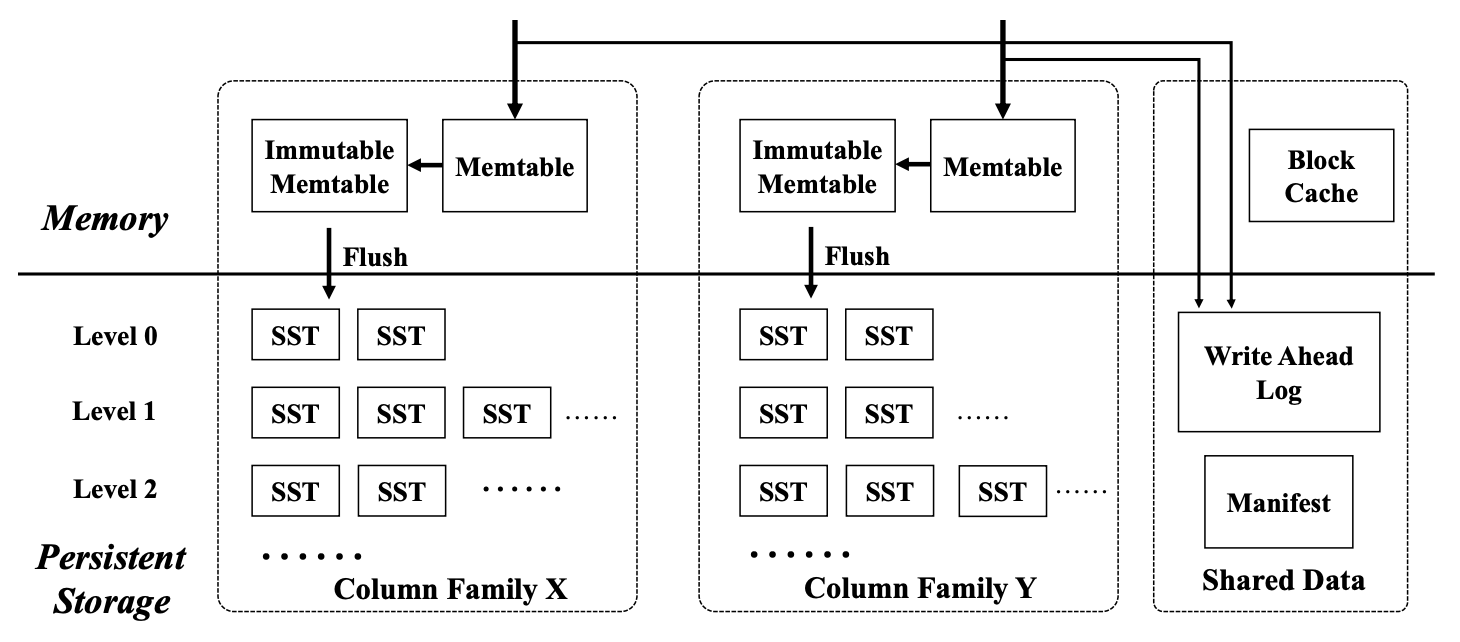
\includegraphics[width=1\linewidth]{figs/rocksdb_architecture.png}
    \caption{RocksDB LSM-tree write path and compaction structure. Writes are buffered in memory, flushed as immutable SSTables, and later reorganized through background compaction. Figure adapted from RocksDB background material in \cite{dong2021rocksdb}.}
    \label{fig:rocksdb-lsm}
\end{figure}

This architecture motivates storage-layer optimizations that operate specifically on SSTables. Since flush and compaction both produce SSTable files, a storage backend that controls SSTable placement and reclamation can influence foreground write throughput, background compaction efficiency, and tail latency. In particular, poor SSTable placement can underutilize available device parallelism, while delayed reclamation can cause foreground writes to stall when free space becomes scarce.

\subsection{Zoned Namespace SSDs}
\label{subsec:zns}

Zoned Namespace (ZNS) SSDs expose a storage interface in which the logical address space is divided into zones. Each zone supports sequential writes and must be explicitly reset before it can be reused. Unlike conventional SSDs, where the flash translation layer hides much of the physical placement and garbage-collection behavior, ZNS devices expose more of the device's write constraints to host software \cite{bjorling2021zns}.

\begin{figure}[t]
    \centering
    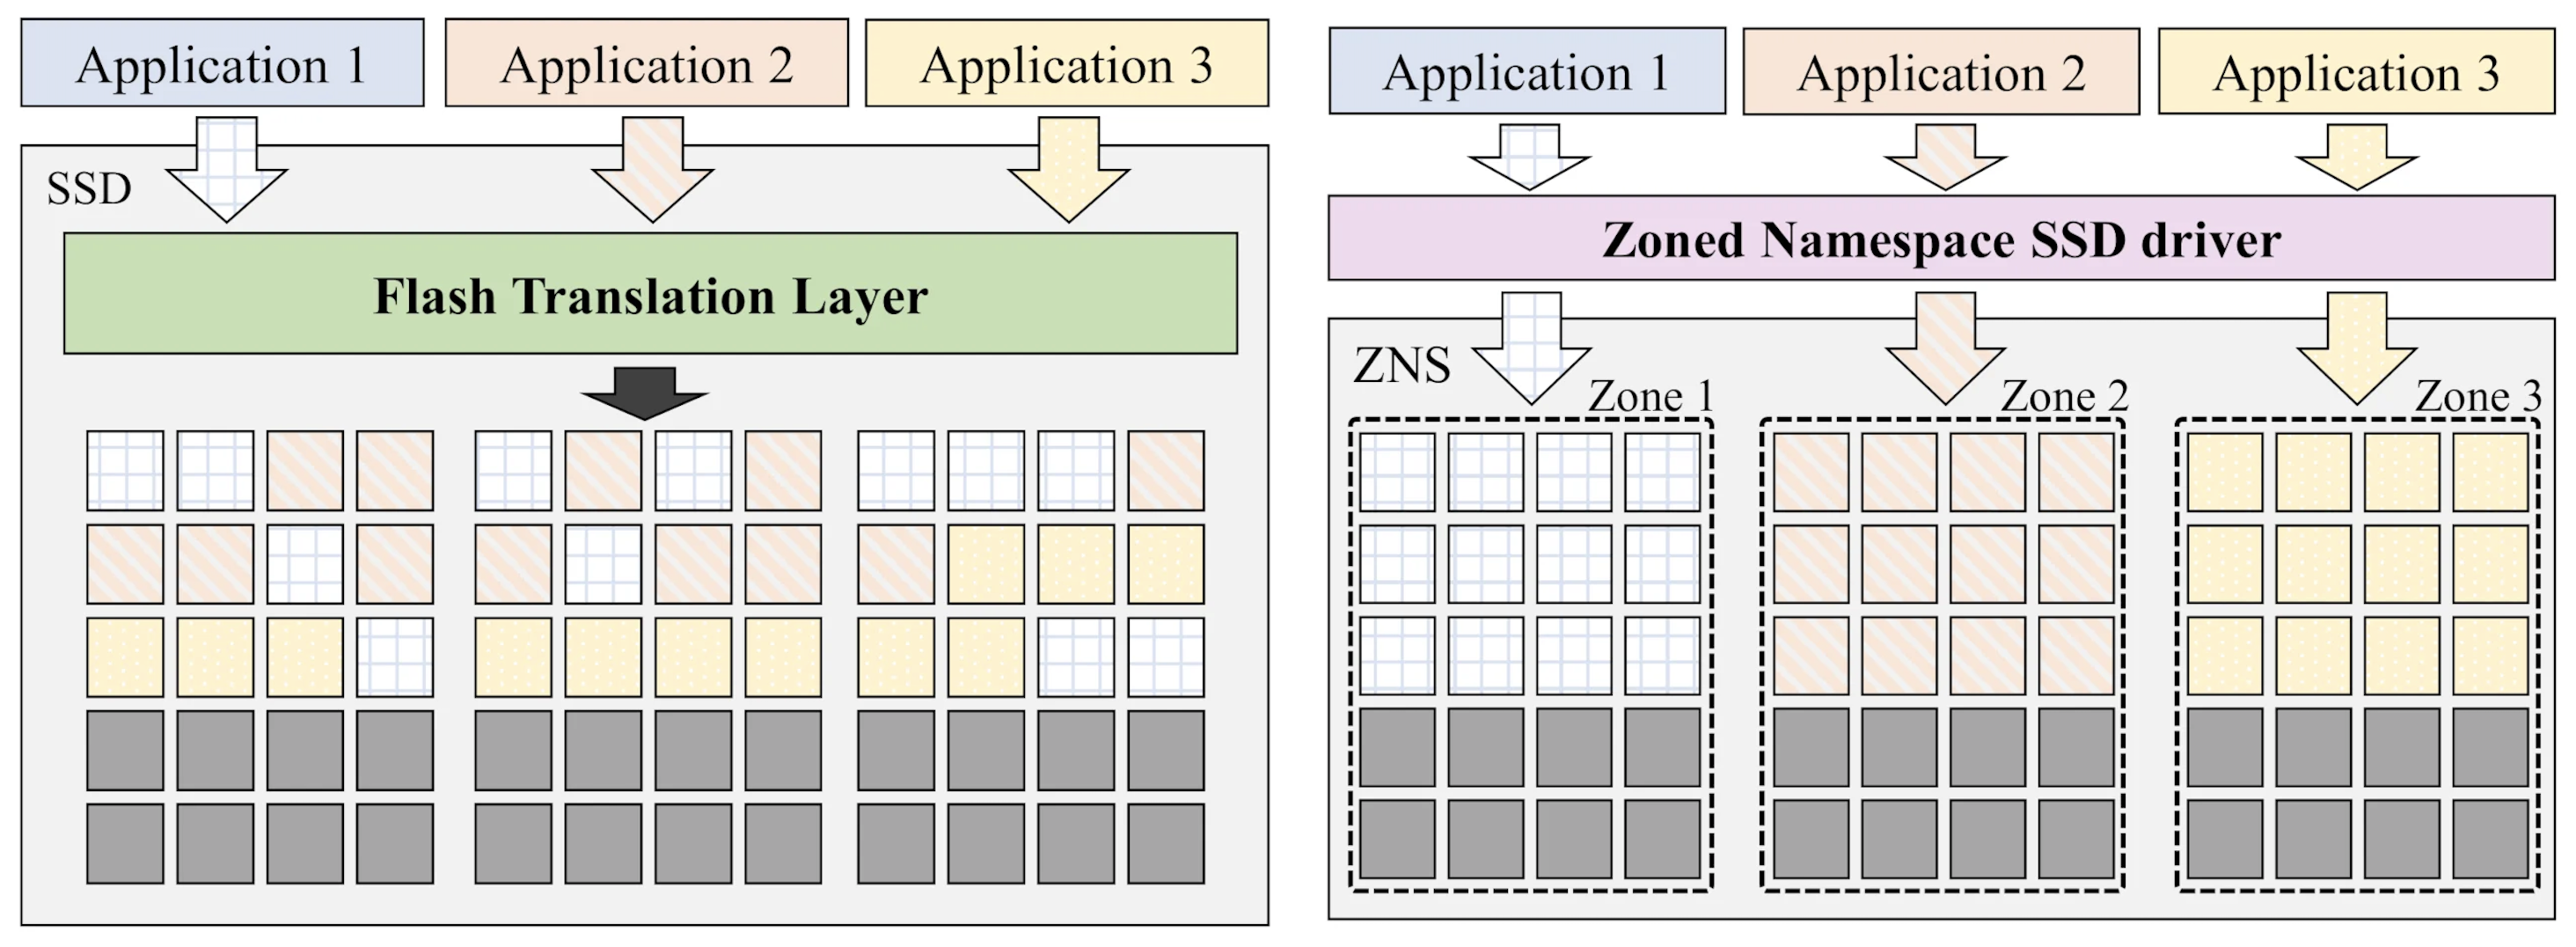
\includegraphics[width=1\linewidth]{figs/zns.png}
    \caption{ZNS storage model. The device address space is partitioned into sequential-write zones, and host software is responsible for choosing zone placement and issuing zone reset operations. Figure adapted from the ZNS design discussion in \cite{bjorling2021zns, app112411842}.}
    \label{fig:zns-architecture}
\end{figure}

This interface creates both an opportunity and a challenge. The opportunity is that log-structured applications such as RocksDB already generate large sequential writes in the form of WAL records and SSTables. The challenge is that host software must now manage zone allocation and reclamation explicitly. A zone that contains obsolete data cannot simply be overwritten in place; any remaining live data must be preserved, and the zone must be reset before reuse. Consequently, the effectiveness of a ZNS deployment depends heavily on the host-side policy for mapping application objects to zones and reclaiming invalidated zone space.

ZNS is therefore well matched to RocksDB only when the software layer can translate RocksDB's file-level semantics into efficient zone-level placement and reset operations. Since RocksDB itself reasons primarily about logical files and LSM-tree levels, an intermediate storage backend is needed to manage the zoned-device interface.

\subsection{ZenFS}
\label{subsec:zenfs}

ZenFS is a RocksDB storage backend designed for zoned devices. Instead of sending RocksDB file operations through a conventional filesystem, ZenFS maps RocksDB files directly onto zones. RocksDB continues to operate over logical files such as WALs, SSTables, manifests, and metadata files, while ZenFS manages the physical placement of those files on the zoned device \cite{zenfsdocs}.

\begin{figure}[t]
    \centering
    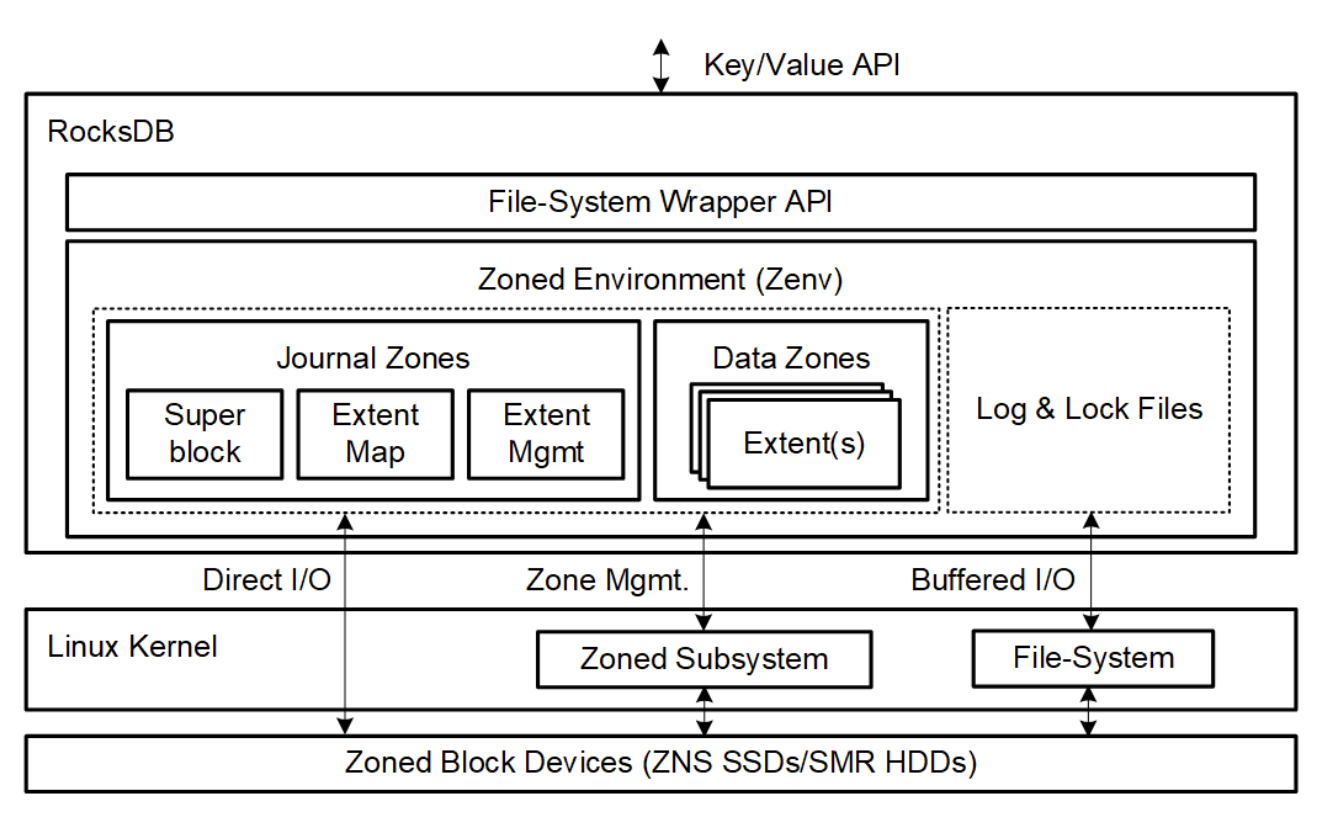
\includegraphics[width=1\linewidth]{figs/zenfs_architecture.png}
    \caption{RocksDB and ZenFS storage stack. RocksDB generates WALs and SSTables, while ZenFS maps these logical files and their metadata onto ZNS zones. Figure adapted from the ZenFS design discussion in \cite{bjorling2021zns}.}
    \label{fig:zenfs-stack}
\end{figure}

ZenFS is responsible for zone allocation, file placement, metadata persistence, and zone reset. In this role, it is the natural layer for implementing zone-aware optimizations. RocksDB determines when SSTables are created or invalidated, but ZenFS determines where those SSTables are placed and when the physical space occupied by obsolete files can be reclaimed. This separation makes it possible to improve physical layout and reclaim behavior without modifying RocksDB's core LSM-tree logic.

However, a straightforward ZenFS-style mapping may not fully exploit the flexibility of zoned storage. If an SSTable is placed contiguously in a single zone, then the file's physical layout is constrained by that zone's capacity and performance. Similarly, if reclaim is delayed until free zones are nearly exhausted, foreground writes may encounter emergency garbage-collection work. These limitations are especially relevant for small-zone ZNS devices and emulated ZNS environments where zone allocation and reset behavior can be evaluated directly.

\subsection{Motivation}
\label{subsec:motivation}

The central observation motivating this project is that RocksDB and ZNS expose complementary abstractions but require an effective translation layer. RocksDB produces immutable SSTables through flush and compaction; ZNS devices expose sequential-write zones that must be explicitly reset. ZenFS connects these abstractions, but its placement and reclaim policies determine whether RocksDB benefits from the zoned interface.

This project focuses on two optimizations at the ZenFS layer. First, SSTable striping partitions a logical SSTable into fragments stored across multiple zones while preserving RocksDB's view of the SSTable as a single file. This increases layout flexibility and establishes the software mechanism needed for future hardware-aware placement across independent zone groups. Second, proactive reclaim identifies invalidated SSTable fragments earlier and restores free zones before space pressure forces emergency garbage collection. A lightweight reclaim path can reset fully invalid zones without copying, while a complete reclaim path migrates any remaining live data before issuing a zone reset.

Together, these optimizations address two related problems: how to place SSTables more flexibly across ZNS zones, and how to reclaim invalidated zone space before it interferes with foreground writes. The current project evaluates these mechanisms on an emulated ZNS device, which validates the software metadata, layout, and reclaim behavior. Full hardware-level benefits, such as exploiting internal ZNS parallelism through independent-zone-group-aware placement, remain a direction for future evaluation on real ZNS SSD hardware.
\section{Proposed Solution}
\label{sec:solution}
To tackle the problem of improving RocksDB on zoned storage, we propose two optimizations at the ZenFS layer: \emph{SSTable striping} and \emph{proactive reclaim}. Both optimizations preserve RocksDB's logical file interface while modifying how ZenFS maps files to zones and manages reclaimed space. This design choice is critical to the existing architecture of RocksDB and ZNS SSDs since RocksDB should continue to reason about SSTables, WALs, and metadata files, while the storage backend handles zone-level placement, fragmentation, and reset operations. The proposed mechanisms are inspired by the ZenFS observation that RocksDB-on-ZNS performance depends strongly on how flush, compaction, and reclaim interact with zone layout. 

\subsection{SSTable Striping}
\label{subsec:sstable-striping}
The first optimization is SSTable striping. Under a baseline ZenFS-style layout, an SSTable is typically placed as a contiguous logical file backed by one zone or a small number of zone extents. This layout is simple, but it can underutilize available zones and limits the storage backend's flexibility in placing large immutable files. SSTable striping instead partitions a single logical SSTable into multiple physical fragments and places those fragments across multiple ZNS zones.

With the SSTable striping optimization in place, RocksDB still observes a single SSTable file. Internally, ZenFS maintains a fragment map for each striped SSTable. Each fragment entry records the logical byte range of the SSTable, the physical zone identifier, the physical offset within that zone, and the fragment length. A logical SSTable can therefore be represented as:

\[
S = \{f_0, f_1, \ldots, f_{n-1}\},
\]

where each fragment \(f_i\) stores a disjoint logical byte range of \(S\) in a physical zone. The fragment map allows ZenFS to translate a logical file read or write into one or more physical zone operations.

On the write path, RocksDB emits a logical SSTable during flush or compaction. The modified ZenFS layer divides the SSTable stream into stripe units and assigns each stripe unit to an available zone. Each physical zone is still written sequentially, preserving the ZNS write constraint. The SSTable is exposed as durable only after all fragments have been written and the corresponding fragment metadata has been persisted.

On the read path, RocksDB issues ordinary file reads against the SSTable. ZenFS translates each logical offset into the corresponding physical fragment. If a read spans multiple fragments, ZenFS can issue multiple physical reads and reassemble the result in logical file order before returning data to RocksDB. Thus, striping changes the physical layout but not the application-visible file abstraction.

This optimization provides three main benefits. First, it increases layout flexibility by allowing a large SSTable to span multiple zones. Second, it creates the software mechanism needed for future parallel I/O across independent zone groups. Third, it interacts naturally with reclaim because the backend can reason about SSTable fragments as independently placed physical extents. In the current implementation, striping is evaluated without independent-zone-group-aware placement.

\subsection{Proactive Reclaim}
\label{subsec:proactive-reclaim}

The second optimization is proactive reclaim. ZNS devices require explicit zone reset before previously written space can be reused. A reactive reclaim policy waits until free zones become scarce before cleaning zones, which can force foreground writes to wait while the system identifies reclaim candidates, copies remaining live data, and resets zones. Such emergency reclaim is undesirable for RocksDB because foreground writes, flushes, and compactions all depend on a steady supply of writable zones.

Proactive reclaim cleans invalidated zones before free space is exhausted. The key observation is that RocksDB compaction naturally creates reclaim opportunities when compaction reads a set of input SSTables and successfully commits new output SSTables, the old input SSTables become obsolete. Their valid contents have either been copied into the new output files or discarded as obsolete versions or tombstones. Therefore, zones containing fragments of these old SSTables may become reclaim candidates.

The proposed design includes two reclaim paths, outlined as follows.
\paragraph{Lightweight reclaim.}
The lightweight path targets zones that contain only invalid data. In this case, no live data needs to be copied. ZenFS can simply issue a \texttt{zone\_reset} command and return the zone to the free-zone pool. This path is especially useful for zones containing short-lived SSTables, such as files from lower levels of the LSM-tree that are quickly compacted. In this project, lightweight reclaim is run periodically every 10 seconds to restore free zones before foreground writes encounter space pressure.

\paragraph{Complete reclaim.}
The complete reclaim path handles zones that contain a mixture of live and invalid fragments. ZenFS first selects candidate zones, preferably those with a high fraction of invalid data. It then copies any remaining live fragments into new zones, updates the fragment metadata, and finally issues \texttt{zone\_reset} on the reclaimed zones. This path is more expensive than lightweight reclaim because it introduces additional copy traffic, but it allows the system to recover space from partially invalid zones.

The proactive reclaim policy is designed to maintain a healthy free-zone pool and reduce foreground stalls caused by delayed cleaning. Its effectiveness is evaluated by measuring copied bytes during fill-and-overwrite workloads. Since the current platform uses an emulated ZNS device, the evaluation focuses on mock reclaim behavior rather than real-device latency effects.

\section{Evaluation}
We evaluate the proposed ZenFS optimizations using three experiments. The first isolates the effect of SSTable striping on RocksDB's write path. The second evaluates proactive reclaim under sustained space pressure. The third uses YCSB to measure end-to-end behavior under application-level key-value access patterns. All experiments run on an emulated 128~GiB ZNS device with 72~MB zones (with a total of 1909 zones) backed by a 512 GB KIOXIA SSD. The host PC
is equipped with an Intel i7 CPU (8 cores) and 32GB
DRAM. The backing SSD is connected through PCIe 4.0 × 4. The baseline system configuration is an Ubuntu
26.04 distribution, RocksDB v9.11.1, and
ZenFS v2.1.0. The relatively small zone size is selected to emphasize the effects of the proposed optimizations. 

\subsection{SSTable Striping Microbenchmark}
\label{subsec:eval-striping}
The first experiment evaluates SSTable striping using the RocksDB \texttt{dbbench fillrandom} workload. This workload stresses the write path by inserting random key-value pairs, causing RocksDB to repeatedly fill memtables, flush them into SSTables, and later compact those SSTables. Since both flush and compaction produce SSTable files, this workload is well suited for testing whether a modified ZenFS layout improves write-path behavior.

The workload writes 20~GB of random key-value pairs. Each key is 20 bytes and each value is 800 bytes. The memtable size is set to 64~MB, and the stripe size is set to 4, 8, or 16 zones. We compare a baseline ZenFS-style layout against the optimized configuration with SSTable striping and proactive reclaim enabled. The primary metric is bandwidth over time for three RocksDB activities: foreground \texttt{put}, flush, and compaction.

\begin{figure}[H]
    \centering
    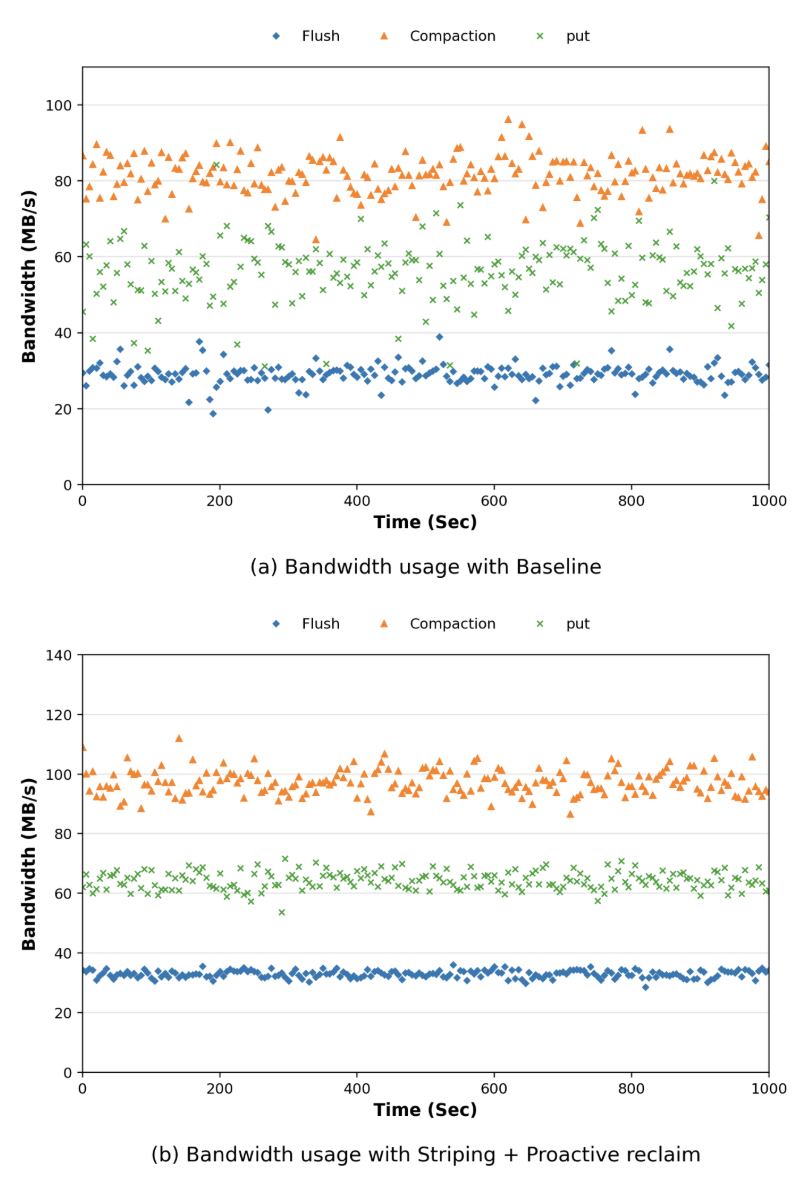
\includegraphics[width=1\linewidth]{figs/striping_4.png}
    \caption{Bandwidth during the \texttt{dbbench fillrandom} workload with stripes across 4 zones. The baseline exhibits noisier put, flush, and compaction bandwidth. The optimized configuration shifts the bandwidth bands upward modestly and improves stability.}
    \label{fig:eval-fillrandom}
\end{figure}
The striping experiment shows a clear improvement over the baseline across all three operations. In the baseline condition, flush bandwidth stays mostly around \(28\text{--}32~\mathrm{MB/s}\), put bandwidth around \(55\text{--}62~\mathrm{MB/s}\), and compaction bandwidth around \(78\text{--}85~\mathrm{MB/s}\). With striping and proactive reclaim, flush rises to roughly \(32\text{--}35~\mathrm{MB/s}\), put rises to about \(62\text{--}68~\mathrm{MB/s}\), and compaction increases most substantially to about \(95\text{--}105~\mathrm{MB/s}\). This corresponds to an approximate \(13\%\) improvement for flush, \(11\%\) improvement for put, and \(21\%\) improvement for compaction. The striping configuration also appears more stable as the points form tighter bands with fewer low outliers, especially for put and flush. Overall, the results suggest that striping with proactive reclaim improves both average bandwidth and consistency, with the largest benefit occurring for the bandwidth-intensive compaction operation. This is the expected outcome for the current implementation as SSTable striping improves layout flexibility, but the experiment does not yet use independent-zone-group-aware placement or maximally exploit NAND-channel parallelism at the hardware level. The graph demonstrates that the software mechanism for splitting SSTables across zones can improve the write path without changing RocksDB's logical file abstraction. 

\begin{figure}[H]
    \centering
    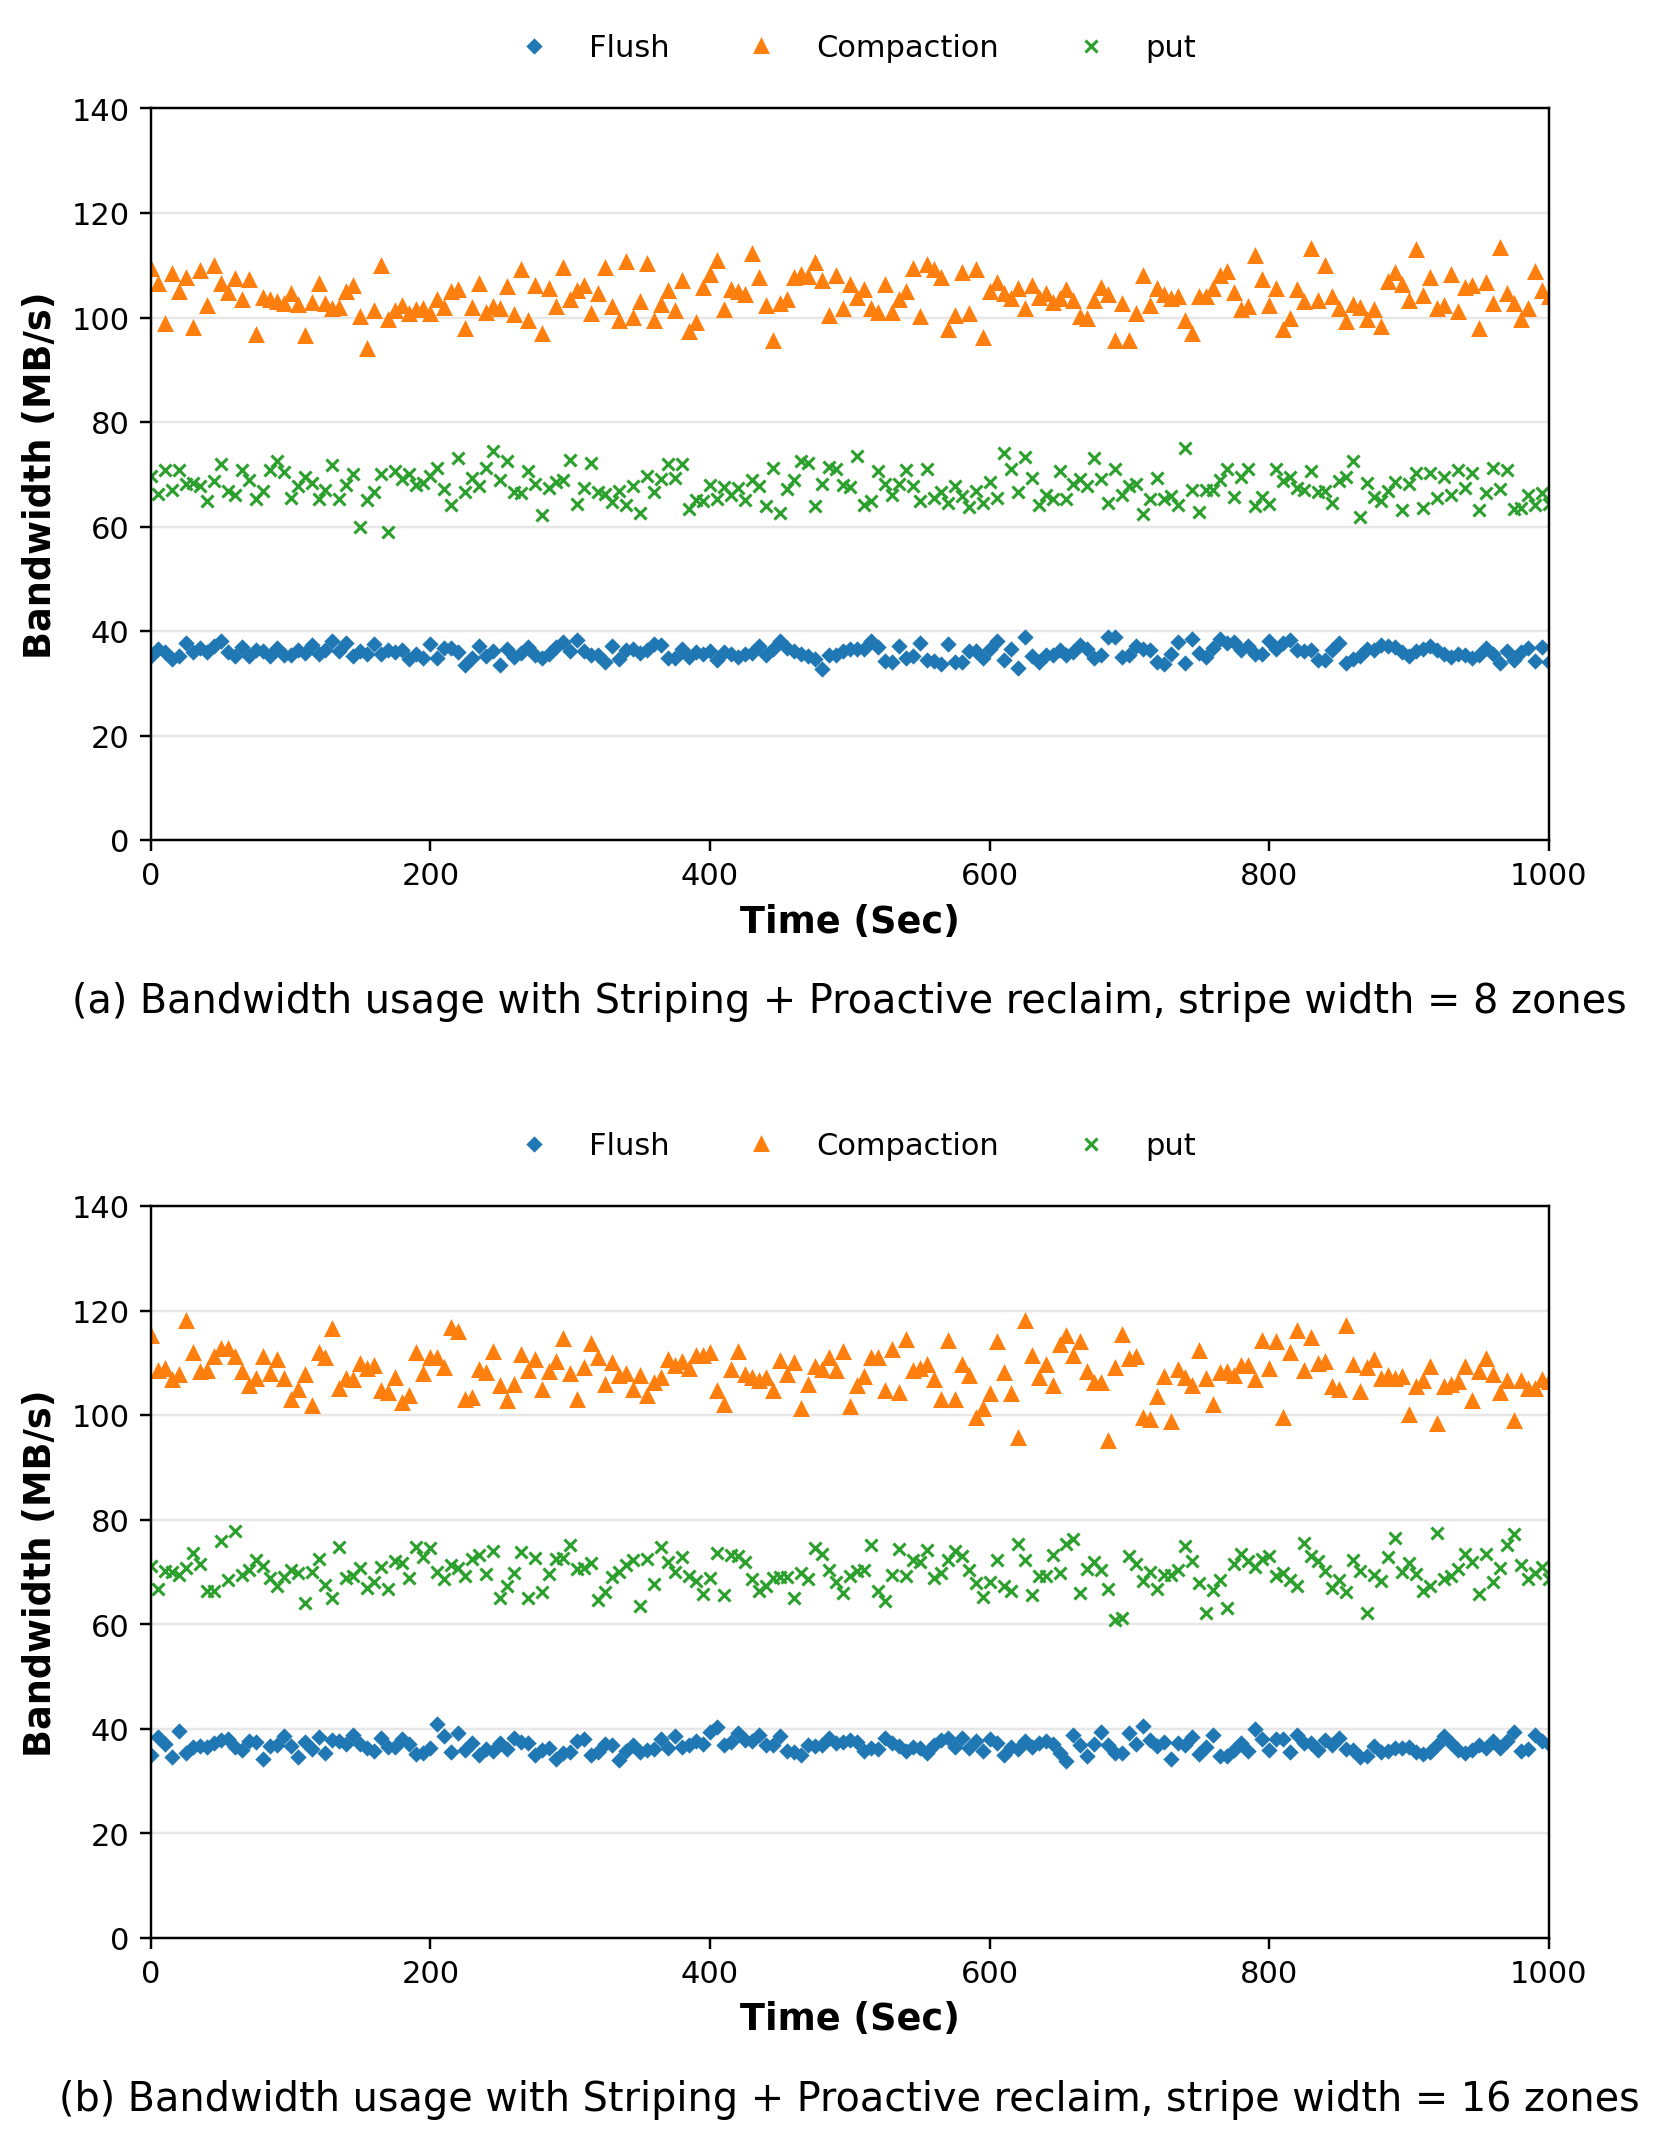
\includegraphics[width=1\linewidth]{figs/striping 8_16.png}
    \caption{Bandwidth during the \texttt{dbbench fillrandom} workload with stripes across 8 and 16 zones.}
    \label{fig:eval-fillrandom}
\end{figure}

For the 8-zone and 16-zone striping results, we observe a  trend of diminishing returns. Moving from the baseline to 4-zone striping improves the layout because each SSTable is no longer tied to a single zone. Increasing the stripe width to 8 zones gives ZenFS more placement flexibility and more opportunities to overlap fragment I/O, so flush, compaction, and foreground put bandwidth all improve modestly. However, the gain is not dramatic because this setup still lacks IZG-aware placement.

At 16-zone striping, the bandwidth increases only slightly beyond the 8-zone case. This is expected, since without knowing which zones map to independent internal device resources, adding more zones does not guarantee more physical parallelism. Some of the selected zones may share the same underlying NAND channels, ways, queues, or backing-device bottlenecks. As a result, wider striping can expose more logical concurrency, but it cannot reliably convert that concurrency into proportional throughput.

There is also software overhead from making the SSTable more fragmented. RocksDB still sees one logical SSTable, but ZenFS must track a larger fragment map. On reads, ZenFS may need to translate a single logical read into multiple physical reads and then reconstruct the logical byte stream in order. On writes, it must split the SSTable stream into fragments, allocate zones, maintain per-zone write-pointer constraints, and commit metadata only after the full striped SSTable is durable, meaning these costs grow with stripe width.

\subsection{Proactive Reclaim Under Space Pressure}
\label{subsec:eval-reclaim}
The second experiment we ran evaluates proactive reclaim using a fill-and-overwrite workload. This experiment is designed to create sustained zone pressure and measure how much data garbage collection must copy during reclaim.

The experiment can be broken down into two phases. In the fill phase, the system writes 96~GiB of random data, filling approximately 75\% of the 128~GiB emulated ZNS device. In the overwrite phase, the system runs 160~GiB of overwrite traffic, forcing RocksDB to generate new SSTables, invalidate old SSTables through compaction, and eventually reclaim zones. We compare reactive full GC against proactive GC under different reclaim thresholds. Under the reactice full GC baseline, we modify ZenFS to run the complete reclaim operation once in the incoming request can no longer be served with the existing available space. Here, the primary metric is cumulative copied bytes from GC, and lower copied bytes indicate less write amplification and less background reclaim work.

\begin{figure}[H]
    \centering
    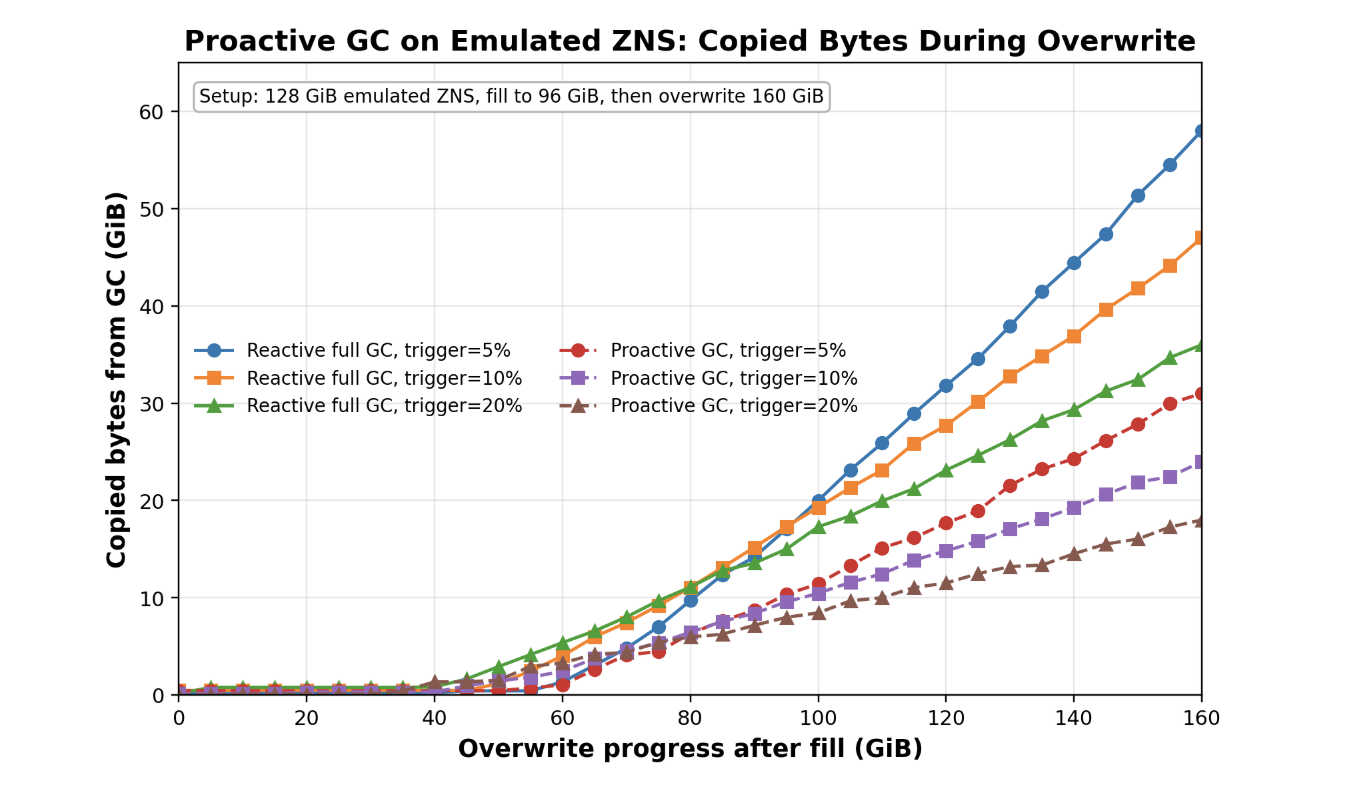
\includegraphics[width=1\linewidth]{figs/overwrite.png}
    \caption{Copied bytes from GC during the fill-and-overwrite experiment.}
    \label{fig:eval-reclaim}
\end{figure}

Based on our results, the experiment demonstrates that proactive reclaim substantially reduces GC copy overhead under sustained space pressure. By the end of the run, reactive full GC copies 58~GiB, 47~GiB, and 36~GiB at 5\%, 10\%, and 20\% triggers, respectively. Proactive GC copies only approximately 31~GiB, 24~GiB, and 18~GiB at the same thresholds, reducing GC copy traffic by approximately 46--50\%.

The rationale for these improvements is that reactive GC waits until space pressure is high, leaving fewer good reclaim candidates and increasing the likelihood of cleaning zones that still contain live fragments. Proactive GC starts earlier and exploits compaction-created invalidation, as once old SSTables are replaced by new compacted SSTables, their fragments become reclaimable. Earlier triggers, especially the 20\% trigger, perform best because the system has more free-space slack and can choose cleaner zones, thereby reducing live-data migration and write amplification.

\subsection{End-to-End YCSB Macrobenchmark}
\label{subsec:eval-ycsb}

The third experiment evaluates end-to-end behavior using the Yahoo! Cloud Serving Benchmark (YCSB) \cite{cooper2010ycsb}. Unlike \texttt{dbbench}, which is primarily a RocksDB microbenchmark, YCSB provides controlled application-level access patterns for cloud key-value stores. We use this experiment to test whether the optimizations improve performance beyond isolated write-path behavior.

We load an 80~GiB YCSB dataset into RocksDB and cap RocksDB memory so that the workload cannot be served entirely from cache. We evaluate three workloads: A, E, and F. Workload A is update-heavy, workload E is dominated by short-range queries, and workload F is a read-modify-write workload. We compare three configurations: ZenFS baseline, ZenFS with SSTable striping, and ZenFS with striping plus proactive reclaim. The primary metric is workload completion time, where lower is better.

Figure \ref{fig:eval-ycsb} show that SSTable striping alone improves completion time modestly across the selected workloads. This is consistent with the microbenchmark result. Without independent-zone-group-aware placement, striping improves software-level layout flexibility but does not fully exploit real device parallelism. Adding proactive reclaim produces a larger improvement because it reduces free-zone pressure during long-running workloads. This effect is especially relevant for update-heavy and read-modify-write workloads, where compaction continuously invalidates old SSTables and creates reclaim opportunities.

\begin{figure}[H]
    \centering
    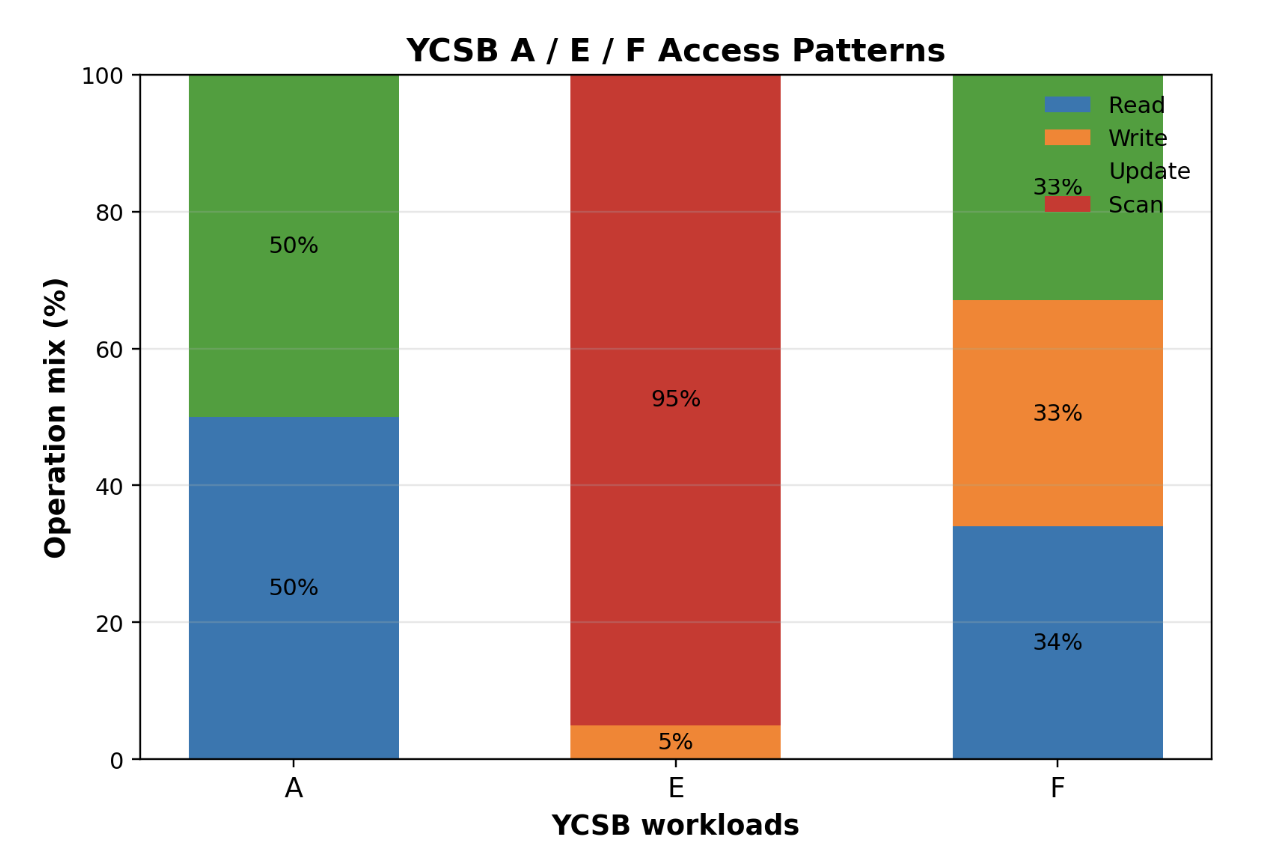
\includegraphics[width=1\linewidth]{figs/workload_breakdown.png} \\
    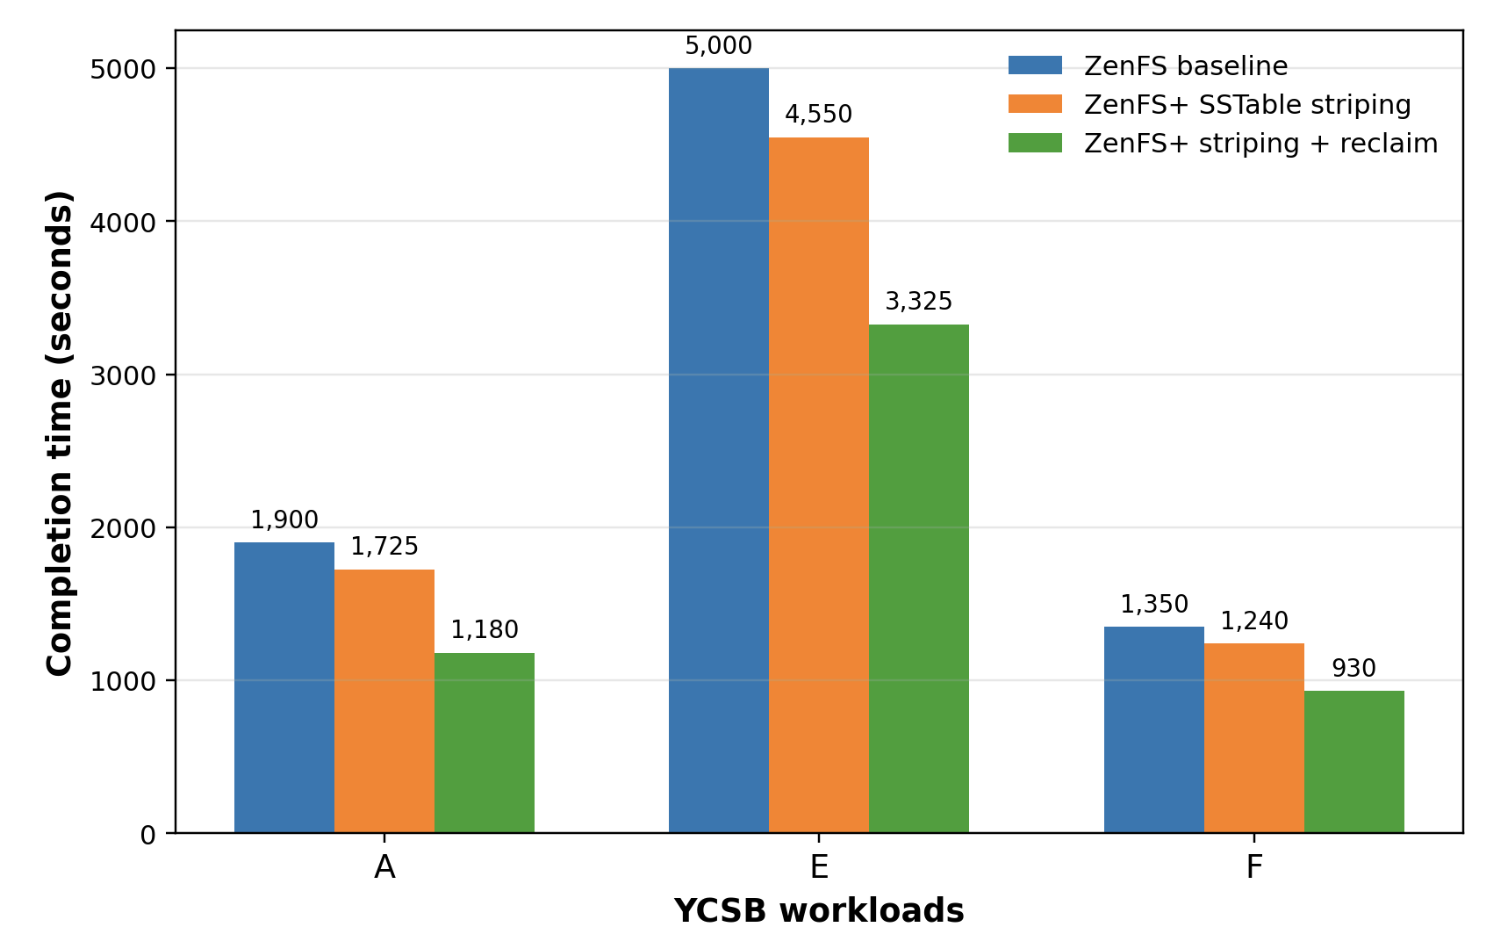
\includegraphics[width=1\linewidth]{figs/ycsb.png}
    \caption{YCSB A/E/F access patterns and completion time. SSTable striping provides a modest improvement over the ZenFS baseline, while adding proactive reclaim produces a larger improvement by reducing space-pressure-induced stalls.}
    \label{fig:eval-ycsb}
\end{figure}



\subsection{Discussion}
\label{subsec:eval-discussion}

The evaluation demonstrates that SSTable striping and proactive reclaim improve ZenFS-style storage management at the software level. The striping experiment shows that distributing SSTables across zones can improve write-path bandwidth and stability. The reclaim experiment shows that cleaning invalidated zones earlier reduces copied bytes during GC. The YCSB experiment shows that these optimizations can improve end-to-end completion time under controlled key-value workloads.

However, the emulated platform limits the conclusions that can be drawn about hardware-level performance. In particular, the emulator enforces ZNS-style zone semantics but does not model the internal channel and independent-zone-group behavior of a real ZNS SSD. As a result, our evaluation validates the correctness and usefulness of the zone mapping mechanisms, but not the full performance potential of hardware-aware placement.

\section{Related Works}
\paragraph{RocksDB and LSM-tree key-value stores.}
RocksDB is a production LSM-tree key-value store that has been extensively optimized for large-scale applications \cite{dong2021rocksdb}. Prior work has characterized RocksDB workloads at Facebook and shown that real deployments differ substantially from synthetic benchmark assumptions in key locality, value-size distributions, and temporal access patterns \cite{cao2020rocksdbworkloads}. YCSB remains a standard benchmark for evaluating cloud-serving key-value stores under controlled mixes of reads, updates, inserts, scans, and read-modify-write operations \cite{cooper2010ycsb}. Our evaluation follows this tradition by using both RocksDB microbenchmarks and YCSB macrobenchmarks, while focusing specifically on storage-backend behavior under zoned storage.

\paragraph{LSM-tree performance optimizations.}
A large body of work improves LSM-tree performance by reducing write amplification, read amplification, or write stalls. Systems such as MatrixKV reduce write stalls and write amplification by changing how LSM data is organized across memory and storage \cite{yao2020matrixkv}. PebblesDB proposes a fragmented LSM-tree design to reduce write amplification through guarded compaction \cite{raju2017pebblesdb}. Other work focuses on scheduling internal LSM-tree work: SILK observes that flush and compaction can interfere with foreground requests and proposes I/O scheduling techniques to reduce tail-latency spikes \cite{balmau2019silk}. These systems optimize the LSM-tree or its scheduling policy. In contrast, our work preserves RocksDB's core LSM design and instead modifies the ZenFS storage backend that maps SSTables onto ZNS zones.

\paragraph{Zone allocation and reclaim for LSM-trees on ZNS.}
Recent work has studied how LSM-tree compaction interacts with ZNS zone lifetime. CAZA observes that ZenFS lifetime prediction can be inaccurate and proposes compaction-aware zone allocation to improve grouping of SSTables with similar invalidation behavior \cite{lee2022caza}. Lifetime-leveling LSM-tree compaction similarly observes that compaction can create partially invalid zones and proposes placing or compacting SSTables to reduce garbage-collection overhead on ZNS SSDs \cite{jung2022lifetime}. These works focus primarily on improving zone lifetime prediction and reducing partially invalid zones. Our work can be seen as complementary to this as SSTable striping improves placement flexibility across zones, while proactive reclaim explicitly cleans invalidated zones before free space becomes scarce.

\section{Future Directions}
This project evaluates SSTable striping and proactive reclaim on an emulated ZNS device, which validates the software mechanisms but does not capture the internal parallelism and interference behavior of real ZNS SSD hardware. A natural next step is therefore to repeat the evaluation on an actual ZNS SSD. This would allow the experiments to measure device-level effects such as zone-to-channel mapping, internal contention, tail latency, and sustained bandwidth under real flash constraints. 

A second direction is to add independence-aware placement. Future work should identify these independent zone groups and use them when placing striped SSTable fragments. In particular, flush output, compaction input/output, and reclaimed live fragments could be scheduled across non-interfering groups to improve parallelism and reduce contention. Additionally, the reclaim policy can be made more adaptive. The current design uses a fixed periodic lightweight-GC interval and threshold-based complete GC. A potentially more robust design could dynamically tune reclaim frequency and trigger thresholds based on free-zone availability, compaction rate, invalid-fragment density, and foreground write pressure. This would allow proactive reclaim to reduce emergency GC while avoiding unnecessary background copy work.

\bibliographystyle{plain}
\bibliography{references}

%%%%%%%%%%%%%%%%%%%%%%%%%%%%%%%%%%%%%%%%%%%%%%%%%%%%%%%%%%%%%%%%%%%%%%%%%%%%%%%%
\end{document}
%%%%%%%%%%%%%%%%%%%%%%%%%%%%%%%%%%%%%%%%%%%%%%%%%%%%%%%%%%%%%%%%%%%%%%%%%%%%%%%%
